% define \title (only used by writelatex.com)
%\title{CSEC-793 Project Report_Blank}
%%%%%%%%%%%%%%%%%%%%%%%%%%%%%%%%%%%%%%%%%%%%%%%%%%%%%%%%%%%%%%%%%%%%%%
% LaTeX Template: Project Titlepage
%
% Source: http://www.howtotex.com
% Date: April 2011
% 
% This is a title page template which be used for articles & reports.
% 
% Feel free to distribute this example, but please keep the referral
% to howtotex.com
% 
%%%%%%%%%%%%%%%%%%%%%%%%%%%%%%%%%%%%%%%%%%%%%%%%%%%%%%%%%%%%%%%%%%%%%%
% How to use writeLaTeX: 
%
% You edit the source code here on the left, and the preview on the
% right shows you the result within a few seconds.
%
% Bookmark this page and share the URL with your co-authors. They can
% edit at the same time!
%
% You can upload figures, bibliographies, custom classes and
% styles using the files menu.
%
% If you're new to LaTeX, the wikibook is a great place to start:
% http://en.wikibooks.org/wiki/LaTeX
%
%%%%%%%%%%%%%%%%%%%%%%%%%%%%%%%%%%%%%%%%%%%%%%%%%%%%%%%%%%%%%%%%%%%%%%
%
% --------------------------------------------------------------------
% Preamble
% --------------------------------------------------------------------
\documentclass[ fontsize=11pt,twoside]{scrartcl}	% KOMA

\usepackage[letterpaper,pdftex]{geometry}	% A4paper margins
\setlength{\oddsidemargin}{5mm}			% Remove 'twosided' indentation
\setlength{\evensidemargin}{5mm}

\usepackage[english]{babel}
\usepackage[protrusion=true,expansion=true]{microtype}	
\usepackage{amsmath,amsfonts,amsthm,amssymb}
\usepackage{graphicx}
\usepackage{pseudocode}

\usepackage[latin1]{inputenc}
\usepackage{tikz}
\usetikzlibrary{shapes,arrows}


% --------------------------------------------------------------------
% Definitions (do not change this)
% --------------------------------------------------------------------
\newcommand{\HRule}[1]{\rule{\linewidth}{#1}} 	% Horizontal rule

\makeatletter							% Title
\def\printtitle{%						
    {\centering \@title\par}}
\makeatother									

\makeatletter							% Author
\def\printauthor{%					
    {\centering \Large \@author}}				
\makeatother							

% --------------------------------------------------------------------
% Metadata (Change this)
% --------------------------------------------------------------------
\title{	\Large \textsc{ CSIT304\\ Fundamentals of Computer Graphics  } 	% Subtitle
		 	\\[2.0cm]								% 2cm spacing
			\HRule{2pt} \\						% Upper rule
			\LARGE \textbf{\uppercase{Project Report
   }}	% Title
			\HRule{2pt} \\ [0.5cm]		% Lower rule + 0.5cm spacing
			\Large \today			% Todays date
		}

 \author{
		Suyash Lal\\	
		School of Computing and Data Sciences\\	
        FLAME University \\
        \texttt{Suyash.lal@flame.edu.in} \\
}


\begin{document}
% ------------------------------------------------------------------------------
% Maketitle
% ------------------------------------------------------------------------------
\thispagestyle{empty}		% Remove page numbering on this page

\printtitle					% Print the title data as defined above
  	\vfill
\printauthor				% Print the author data as defined above
\newpage
% ------------------------------------------------------------------------------
% Begin document
% ------------------------------------------------------------------------------
\setcounter{page}{1}		% Set page numbering to begin on this page


%%%%%%%%%%%%%%%
%														%
% 			Main Contents            %
%														%
%%%%%%%%%%%%%%%

\section{OpenGL}
\subsection{Goal of the Project}
The primary goal of this project is to create a traffic simulation using OpenGL to model and visualize the dynamic behavior of vehicles at a traffic light. This includes simulating different traffic light phases and car movements in response to these phases.

\subsection{Rationale of the Project}
The rationale behind developing a traffic simulation is to somewhat simulate an interaction between object. Since I wanted to implement something with relation to time and action, I came across the thought of a traffic light simulation, where the car will move in accordance to the way the light shifts in color. I've tried to ensure that the traffic light is functioning and the response of the car is the same as the way any disciplined driver would do.

\subsection{Importance of the Project}
This project is important as it has helped me to figure out how to overlay objects over each other, like the number of wheels of the car, along with the windshield. The biggest problem I faced was at the very beginning, where I first created the pole along with the different colors. Fixing them in place and moving them collectively made it easier to create the car. Initially the traffic lights were black and only turned to the color when called, instead I set an initial color of the darkened value of the lit up color. This implementation made it visually more pleasing to look at and see the changed (instead of it turning to the respective colors from a black color state).

\subsection{Main Contributions to the Project}
The main contributions of this project include:
\begin{itemize}
    \item Creating realistic car animations that respond to traffic light changes.
    \item Developing an intuitive visualization of the traffic system which can be used for educational purposes.
    \item With time, creating the stop, slow, and fast effect of the car.
\end{itemize}

\subsection{Screenshots of the Project}
Below are important features of the project captured in screenshots - the traffic light function and the update function of the light states.

\begin{figure}[!htb]
    \centering
    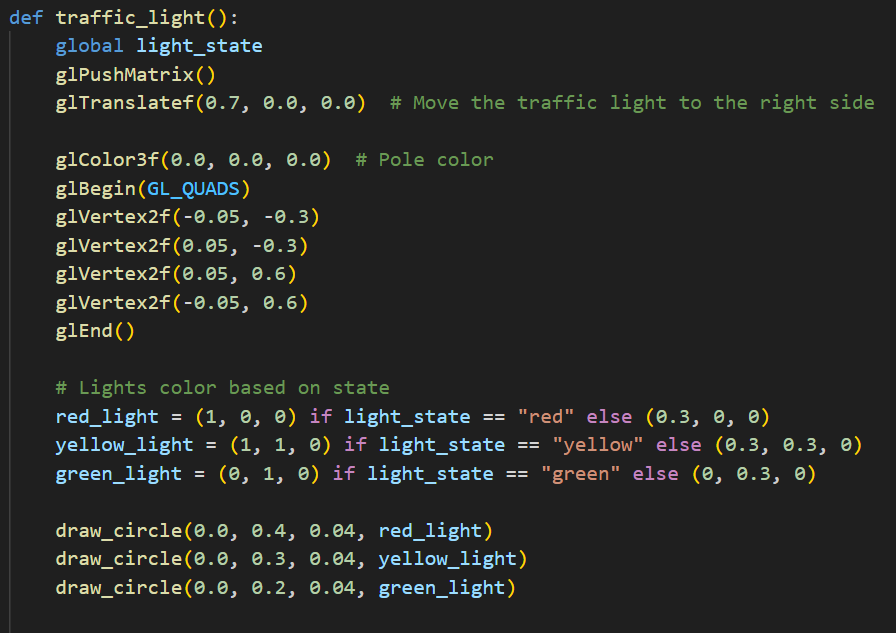
\includegraphics[width=0.8\textwidth]{TrafficLightFunc.png}
    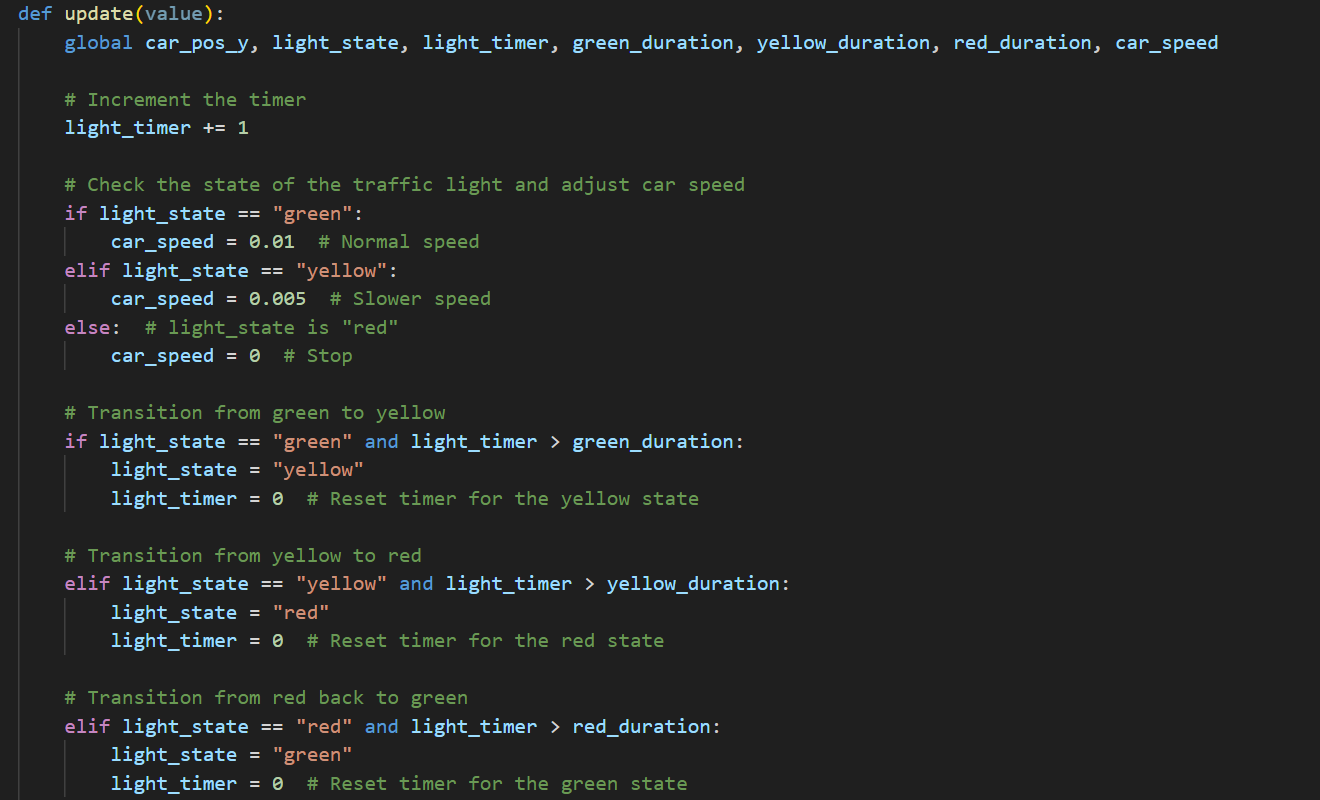
\includegraphics[width=0.8\textwidth]{updatefunc.png}
    \label{fig:traffic_simulation}
\end{figure}

\clearpage

\section{Blender}
\subsection{Goal of the Project}
The primary goal of this project is to create a realistic football simulation using Blender to model and animate dynamic interactions between players and the ball. This simulation aims to demonstrate the capabilities of Blender in creating sports animations and interactions, and to see how I can make objects interact with one another with game physics.

\subsection{Rationale of the Project}
This project was developed to explore Blender's animation and physics simulation capabilities in a controlled sports scenario. By simulating a football being scored, the project demonstrates how Blender can be utilized to animate and understand the physics behind ball movement, which is fundamental in sports animation. I wanted to create more than just this simple animation and actually submitted 2 files, the reason being so the Blender1 file was my first implementation without the help of online sources. The issue I faced was the frequent crashes I experienced after rendering the animation although I was happy with the fact that the animation was working well in the viewport shading mode, whenever I tried the rendered animation, my laptop would crash. At the same time if I packed the textures it would only make the image all the more slower. Due to this, I created a second blender project where I could show the simulation without facing issues like FPS (frames per second) drops, and film grain. The video I referred to is listed in the references section. 

\subsection{Importance of the Project}
The importance of this football goal simulation lies in its simplicity and focus. It also helps me understand how much work goes into UI game design of games like FIFA, NBA2K, and all the other sports games that exist. Since game design is a field that I'm aspiring to go forward in, having a skill in Blender would make it all the more easier to implement new features in the games I make.

\subsection{Main Contributions to the Project}
The main contributions of this project include:
\begin{itemize}
    \item \textbf{Animation:} Developed a fluid animation of a football flying into a goal, capturing the essence of motion and impact.
    \item \textbf{Physics Simulation:} Implemented realistic physics to govern the trajectory, where I turn on animate and create another key frame where I turn it off to set the gravity physics of the ball back, enhancing the visualization of the simulation.
    \item \textbf{Visual Rendering:} Using Blender's rendering tools to create a visually appealing depiction of a football goal scene and interaction. I created the ball and the goalpost with the help of videos for each of them.
\end{itemize}
\subsection{Screenshots of the Project}
Below are the rendered image of both the blender files I made:

    \begin{figure}[!htb]
        \centering
        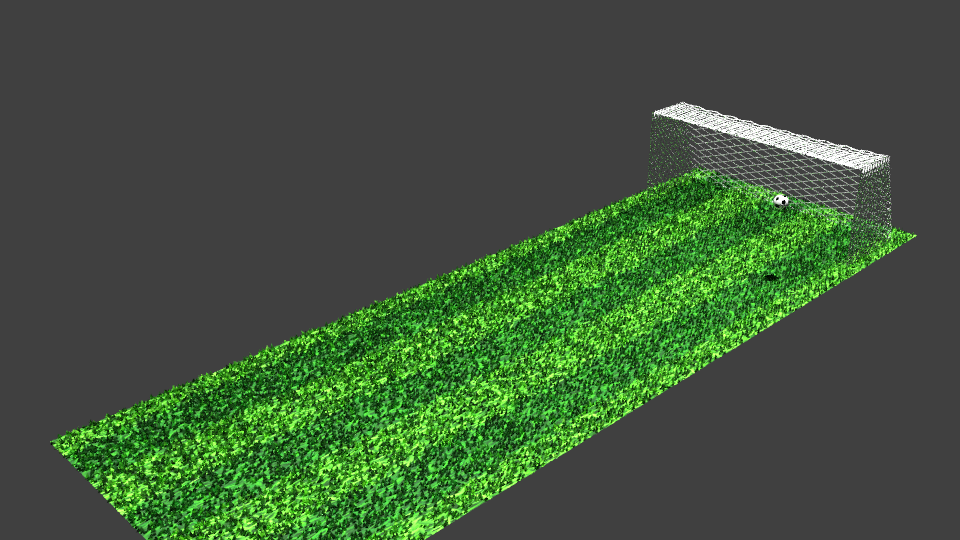
\includegraphics[width=0.8\textwidth]{Blender_1_RenderedImage.png}
        \caption{First implementation}
        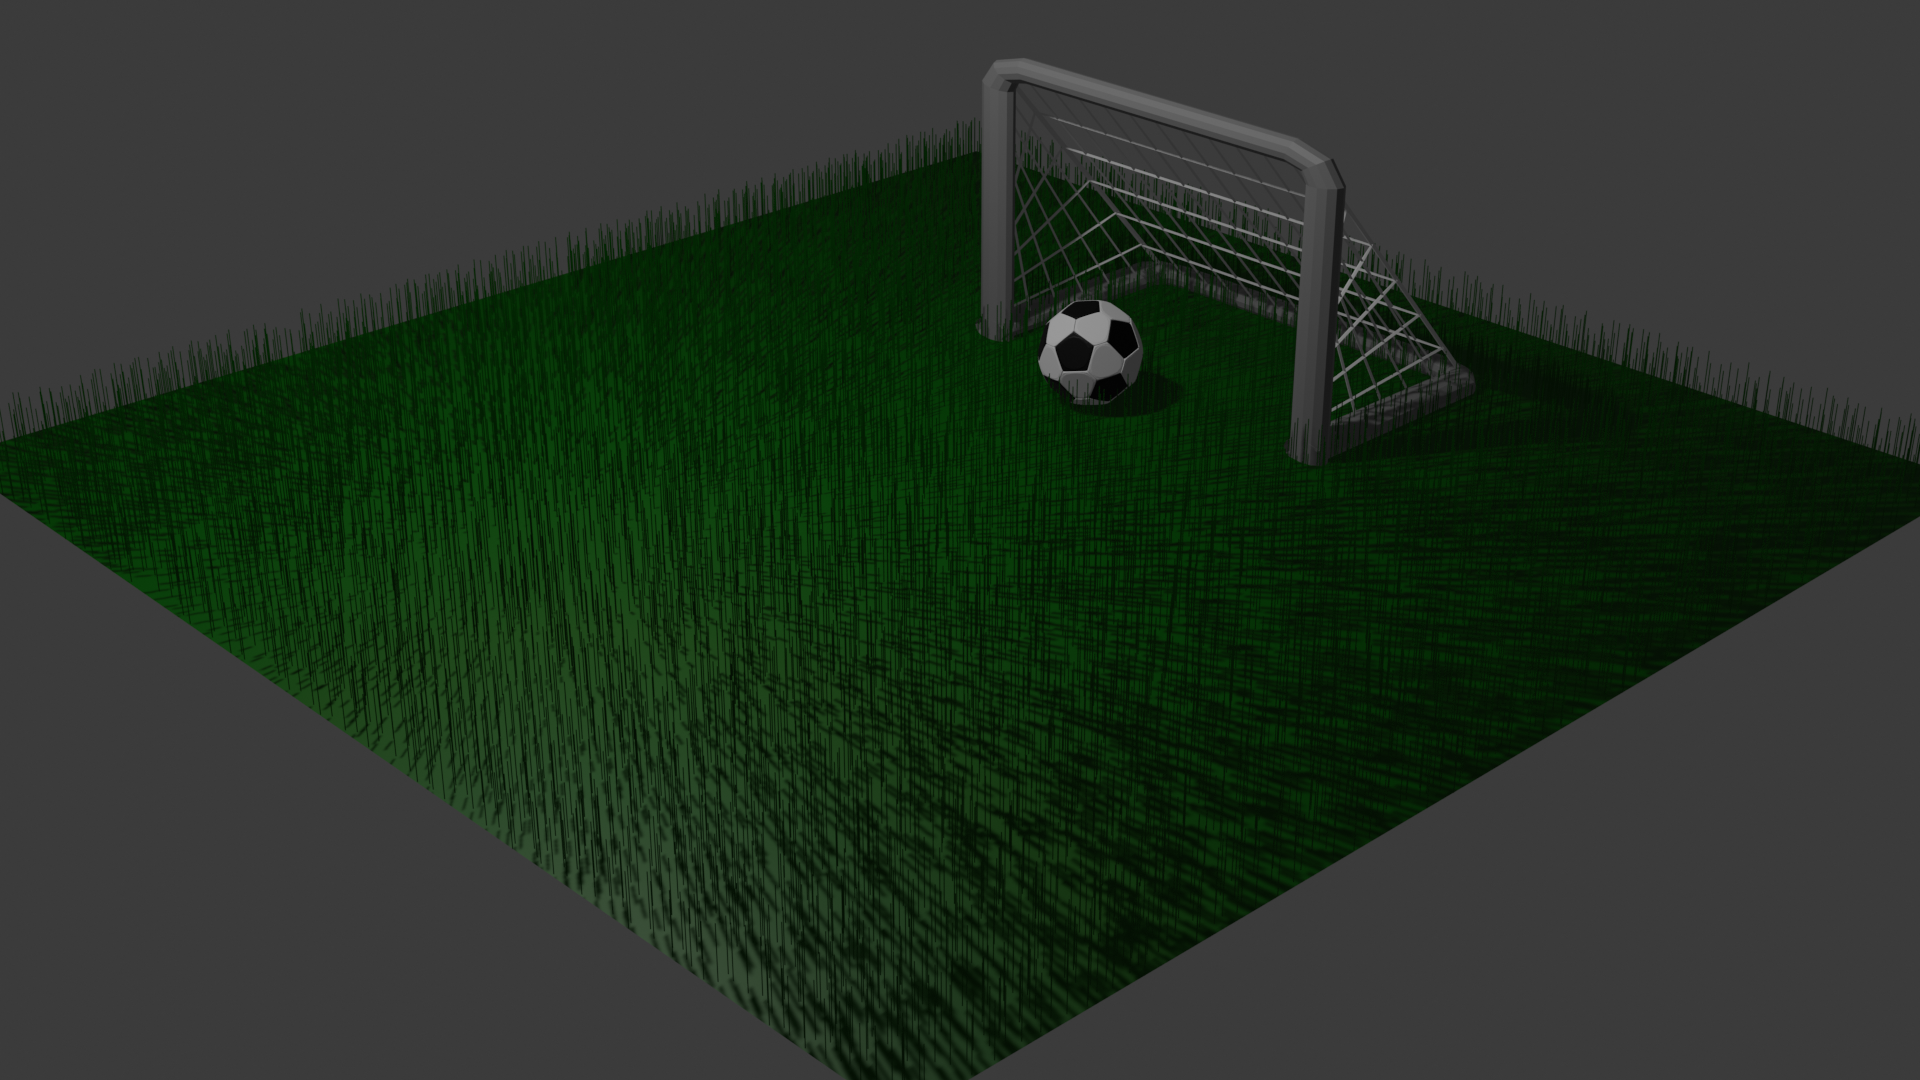
\includegraphics[width=0.8\textwidth]{Blender_2_RenderedImage.png}
        \caption{Second implementation}
        \label{fig:Blender_Renders}
    \end{figure}

\clearpage

\section{Conclusion}

This project in both OpenGL and Blender has significantly enhanced my understanding and capabilities in graphics programming and animation. Through the OpenGL traffic simulation, I learned how to control object behaviors dynamically in response to time-based events, such as traffic lights changing from green to yellow to red. This not only involved graphic rendering but also the synchronization of multiple elements to create a realistic simulation environment.
\newline
\newline
In the Blender football simulation, I tackled different challenges, particularly in rendering and physics simulation, which taught me a great deal about managing resources in animation projects. Both projects allowed me to apply theoretical knowledge in a practical setting, thereby bridging the gap between conceptual learning and real-world application.
\newline
\newline
These experiences are invaluable as they have prepared me for more complex projects in the fields of game development and simulation. The skills acquired, especially in Blender, are directly applicable to UI game design and will undoubtedly aid in my career aspirations in game development.
\newline
\newline
Moreover, the ability to overcome technical challenges, such as system crashes and performance issues, has provided me with a robust problem-solving toolkit. Each project not only pushed the boundaries of my technical skills but also enhanced my creative thinking and project management abilities.

\section{Acknowledgement}
I would like to express my sincere gratitude to Professor Chiranjoy Chattopadhyay, my project supervisor, for their invaluable guidance, patience, and expertise. Their insights and feedback were instrumental in shaping both the direction and execution of this project.

\clearpage

\section{References}
\\
\subsection{First Blender reference video - each object creation}

\subsubsection{Grass creation}
Author = {Unreal King}
\\
Title = {{How to make grass in 40 seconds! (Blender Tutorial)}}
\\
URL = {https://www.youtube.com/watch?v=oavPuJuRc3E}

\subsubsection{Simulation understand reference}
Author = {Fridqeir}
\\
Title = {{How To Make Goal Net Simulation Blender}}
\\
URL = {https://www.youtube.com/watch?v=XAlHz1XrS2Q}

\subsubsection{Goal post creation}

Author = {KAZMA}
\\
Title = {{Simple Football Goal Post modeling in Blender}}
\\
URL = {https://www.youtube.com/watch?v=NcPUBUiJpR8&t=1s}

\subsection{Second Blender reference video}
Author = {Maba 3D},
\\
Title = {{Lowpoly football goal and ball animation tutorial in Blender|Maba 3D}}
\\
URL = {https://www.youtube.com/watch?v=1MjFwoVT5zs}


% ------------------------------------------------------------------------------
% End document
% ------------------------------------------------------------------------------
\end{document}